%------------------------------------------%
% Cannabis Data Science #85
% Copyright (c) 2022 Cannlytics
% Date: 9/28/2022
%------------------------------------------%
\documentclass[xcolor={dvipsnames}]{beamer}
\hypersetup{pdfpagemode = FullScreen}
\mode<presentation>{
  \usetheme{Boadilla}
  \usecolortheme{orchid}
  \usefonttheme{default}
  \setbeamertemplate{navigation symbols}{}
  \setbeamertemplate{caption}[numbered]
}
\setbeamersize{
  text margin left = 0.5in,
  text margin right = 0.5in
}

%------------------------------------------%
% Title
%------------------------------------------%
\title[\textbf{Cannabis Data Science \#85}]{}
\author{Cannlytics}
\institute[]{\Large Cannabis Data Science \#85}
\date{September \nth{28}, 2022}

%------------------------------------------%
% Packages
%------------------------------------------%
\usepackage[english]{babel}
\usepackage[utf8x]{inputenc}
\usepackage{tikz} % For styling.
\usepackage{xparse}
\usepackage{amsmath}
\renewcommand*\footnoterule{} % No footnote line.
\usepackage{mathtools} % Annotating equations.
\usepackage{hhline} % Double bars.
\usepackage[super]{nth} % 1st, 2nd, 3rd, etc.
\usepackage{graphicx, caption, subcaption}
\usepackage{setspace}
\usepackage[charter]{mathdesign}
\usepackage{tikz}
\usetikzlibrary{tikzmark}
\usetikzlibrary{arrows.meta}

%------------------------------------------%
% Theme
%------------------------------------------%
\definecolor{LG}{RGB}{218, 247, 166}
\definecolor{DG}{RGB}{2, 48, 32}
\setbeamercolor*{palette primary}{bg=LG, fg=DG}
\setbeamercolor*{palette secondary}{bg=LG, fg=DG}
\setbeamercolor*{palette tertiary}{bg=LG, fg=DG}

%------------------------------------------%
% Commands
%------------------------------------------%

% Top space.
\newcommand\T{\rule{0pt}{2.5ex}}

% Bottom space.
\newcommand\B{\rule[-1.25ex]{0pt}{0pt}}

% Blocks.
\newenvironment<>{Block}[2][.9\textwidth]
  {\setlength{\textwidth}{#1}
  \begin{actionenv}#3
    \def\insertblocktitle{#2}\par
    \usebeamertemplate{block begin}}
  {\par\usebeamertemplate{block end}
  \end{actionenv}}

% Balls.
\defbeamertemplate{enumerate item}{largeball}
{\begin{pgfpicture}{-1ex}{-0.65ex}{1.5ex}{1.5ex}
\usebeamercolor[fg]{item projected}
{\pgftransformscale{2.5}\pgftext{\Large\pgfuseshading{bigsphere}}}
{\pgftransformshift{\pgfpoint{0pt}{0.5pt}}
\pgftext{\usebeamerfont*{item projected}\small\insertenumlabel}}
\end{pgfpicture}}

% Fancy arrows.
\NewDocumentCommand\UpArrow{O{2.0ex} O{black}}{%
   \mathrel{\tikz[baseline] \draw [->, line width=0.5pt, #2] (0,0) -- ++(0,#1);}} % Fancy up-arrow.
\NewDocumentCommand\DownArrow{O{2.0ex} O{black}}{%
   \mathrel{\tikz[baseline] \draw [<-, line width=0.5pt, #2] (0,0) -- ++(0,#1);}} % Fancy down-arrow.

% Equations with numbers on the left.
\makeatletter
\newcommand{\LeftEqNo}{\let\veqno\@@leqno}
\makeatother

% Print out title.
\defbeamertemplate*{title page}{customized}[1][]
{
  \usebeamerfont{title}\inserttitle\par
  \bigskip
  \vspace{0.5\baselineskip}
  \usebeamerfont{institute}\insertinstitute\par
  \vspace{0.5\baselineskip}
  {\small\usebeamerfont{date}\insertdate\par}
  \usebeamercolor[fg]{titlegraphic}\inserttitlegraphic
}

%------------------------------------------%
% Presentation
%------------------------------------------%
\begin{document}

% Title page.
\begin{frame}{}

% Background
\tikz[remember picture, overlay]
\node[opacity=1.0, inner sep=0pt] at (current page.center){
  
\includegraphics[height=\paperheight, width=\paperwidth]{images/presentation-cover.pdf}
};

% Title
\vspace*{4\baselineskip}

\includegraphics[scale=0.375]{images/logo.pdf}
\vspace*{-2\baselineskip}
\titlepage
\end{frame}

%------------------------------------------%
% Introduction
%------------------------------------------%

\begin{frame}{Cannabis Commerce}

\begin{center}
\includegraphics[width=0.5\textwidth]{images/ca-cannabis-fire-map.png}
\end{center}

{\tiny\setstretch{0} Dillis, Christopher, Butsic, Van, Moanga, Diana, Parker-Shames, Phoebe, Wartenberg, Ariani, and Grantham, Theodore E.. 2022. ``The Threat of Wildfire is Unique to Cannabis among Agricultural Sectors in California.'' Ecosphere 13( 9): e4205. https://doi.org/10.1002/ecs2.4205}

\end{frame}

%------------------------------------------%
% Literature Review
%------------------------------------------%

% Page 
\begin{frame}{Literature Review}

\vspace{0.5\baselineskip}
Topics:

\vspace{0.5\baselineskip}
\begin{itemize}

\item California prepares for interstate cannabis commerce.

\vspace{0.5\baselineskip}

\item Kentucky congress members push for FDA CBD oversight.

\vspace{0.5\baselineskip}

\item $\Delta$--8 THC, novel cannabinoids, concentrates, additives.

\end{itemize}

% Picture of COAs.
\vspace{1\baselineskip}
\begin{minipage}{0.45\textwidth}

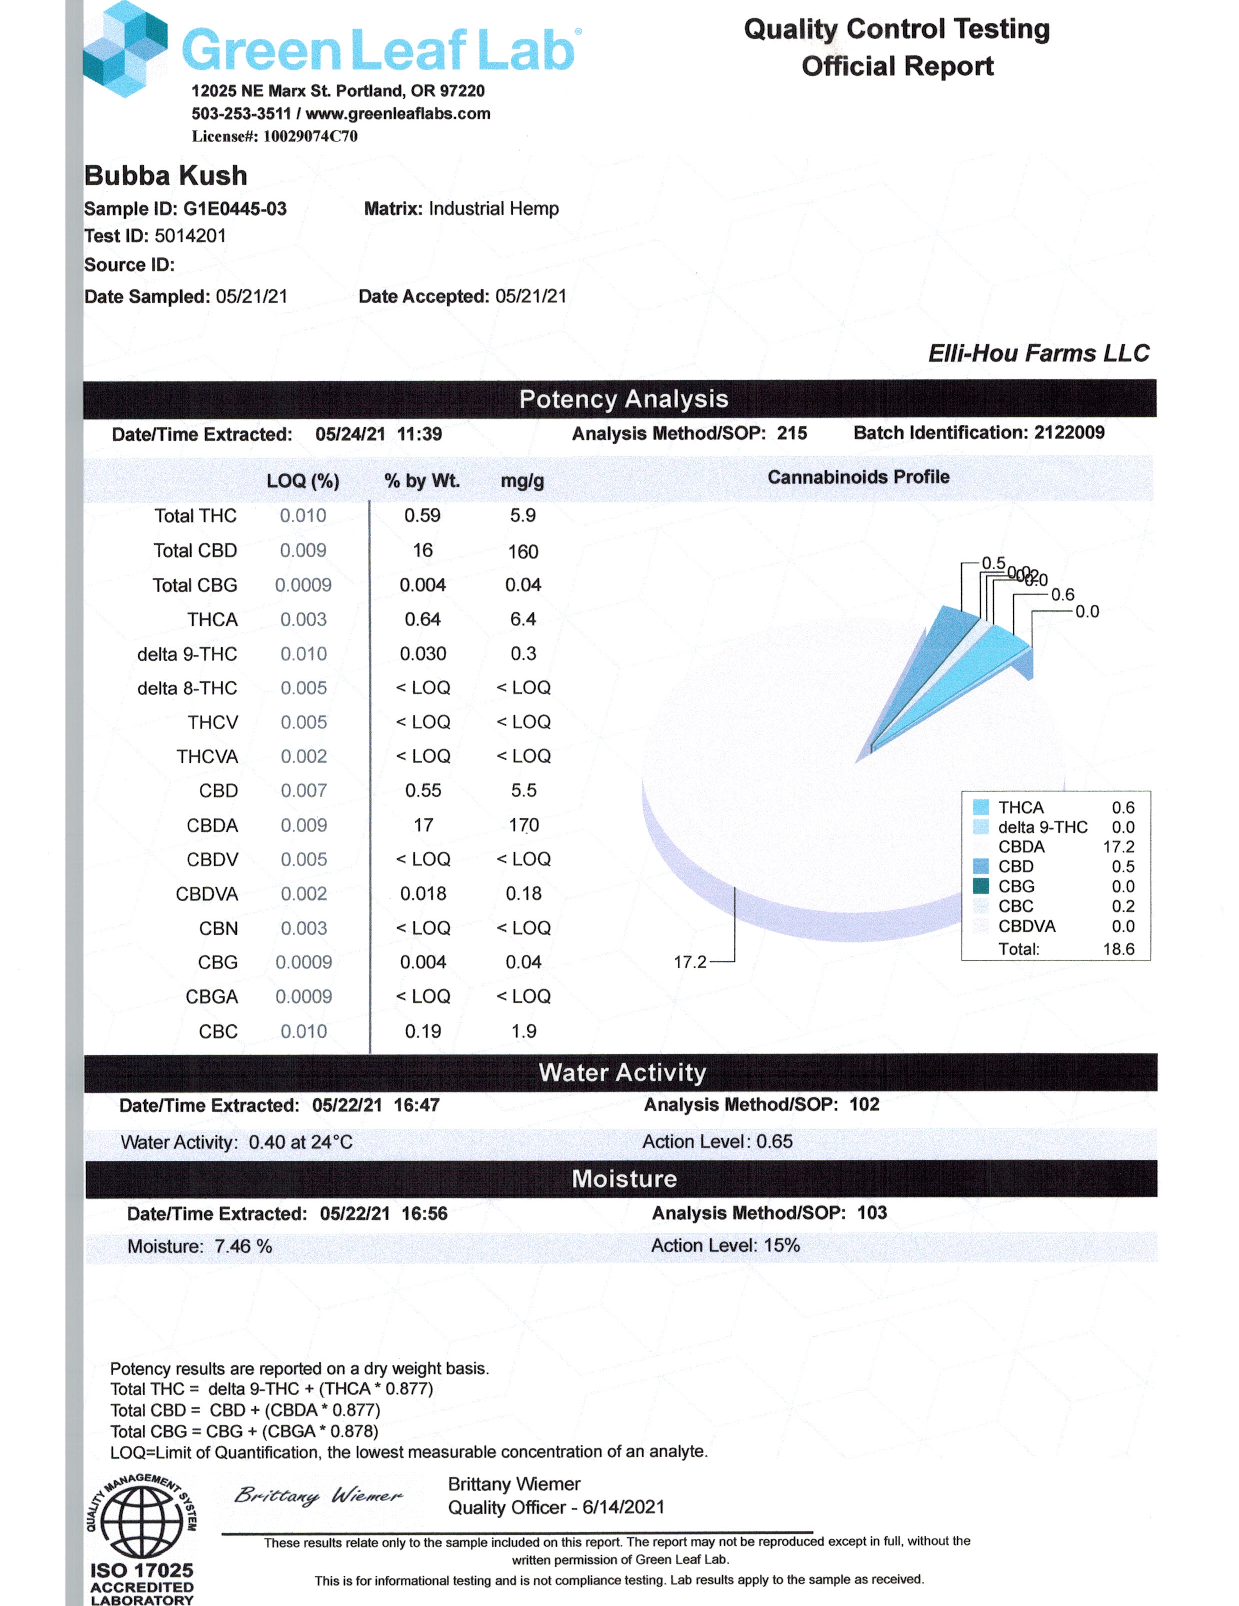
\includegraphics[width=\textwidth]{images/bubba-kush-coa.pdf}

\end{minipage}\hspace{0.045\textwidth}%
\begin{minipage}{0.45\textwidth}

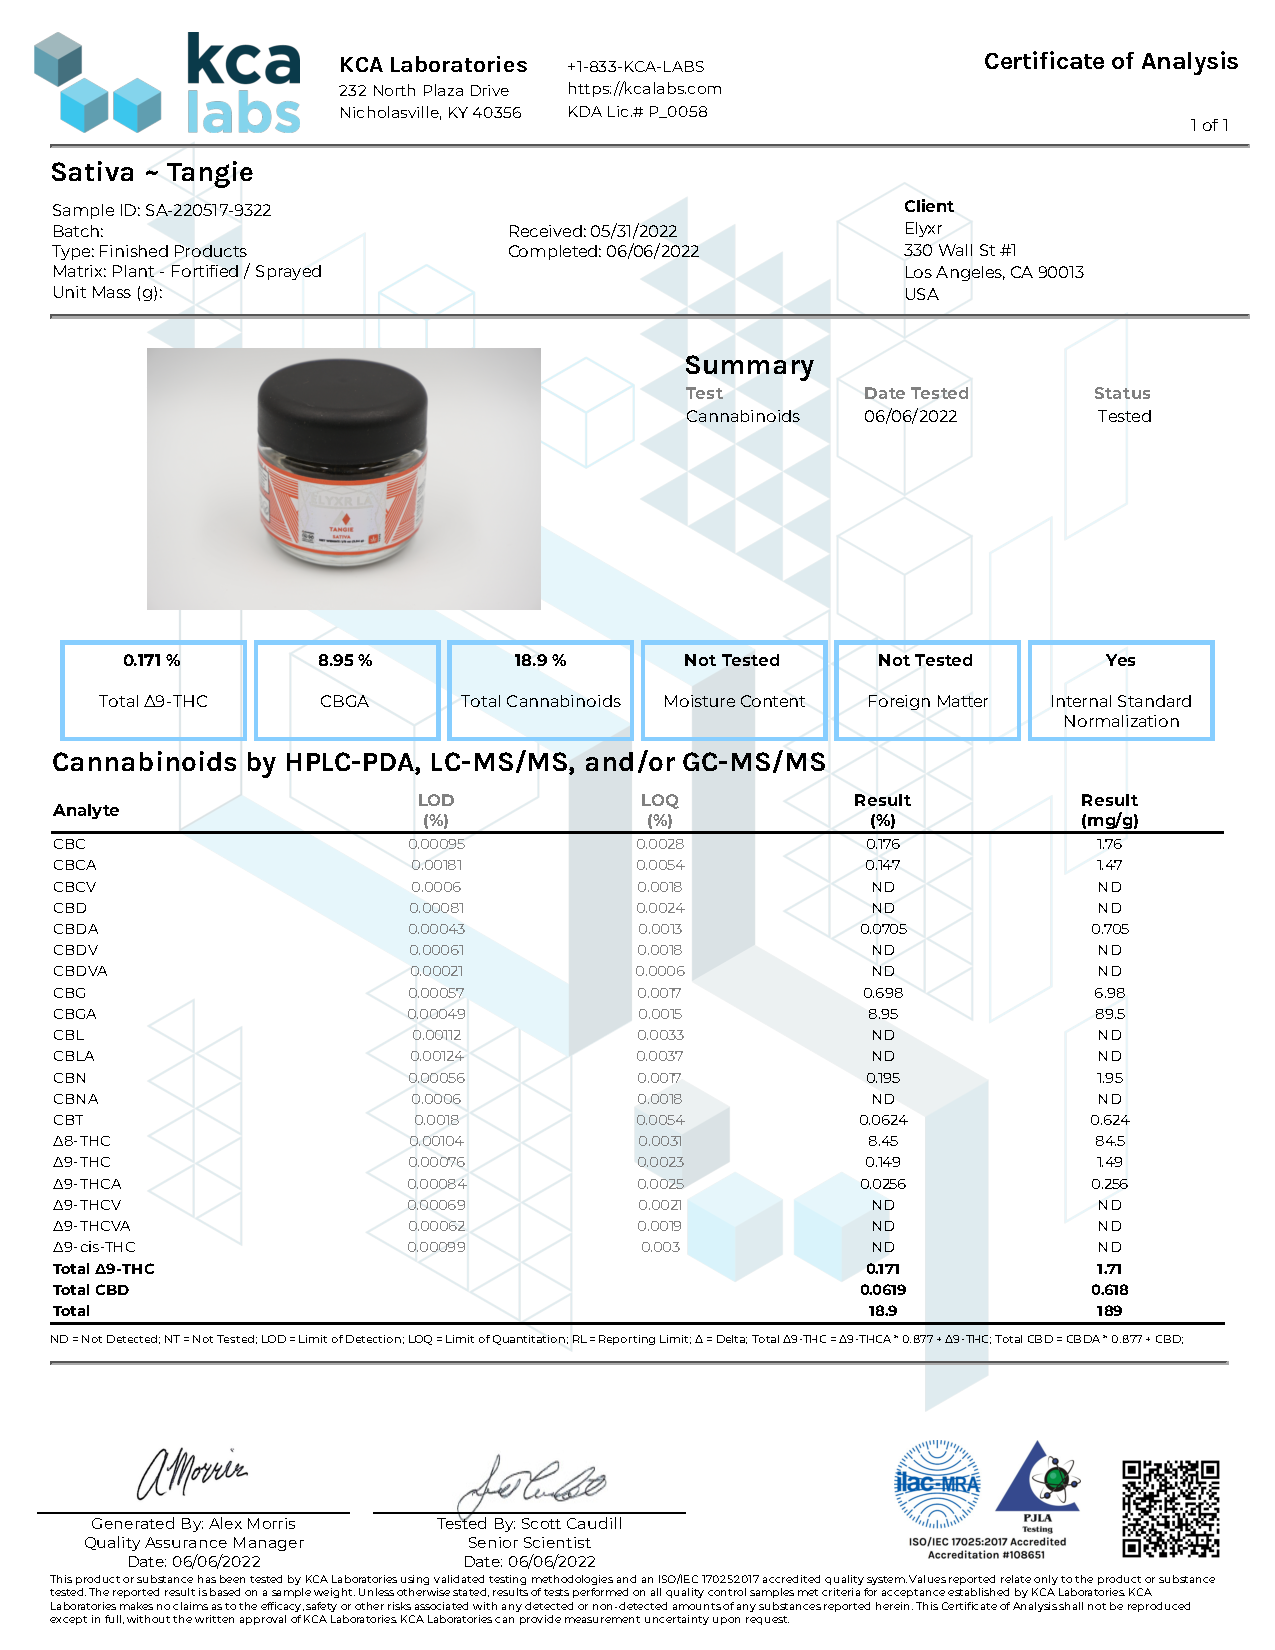
\includegraphics[width=\textwidth]{images/tangie-coa.pdf}

\end{minipage}

\end{frame}

% Page 
\begin{frame}{Literature Review}

\begin{center}
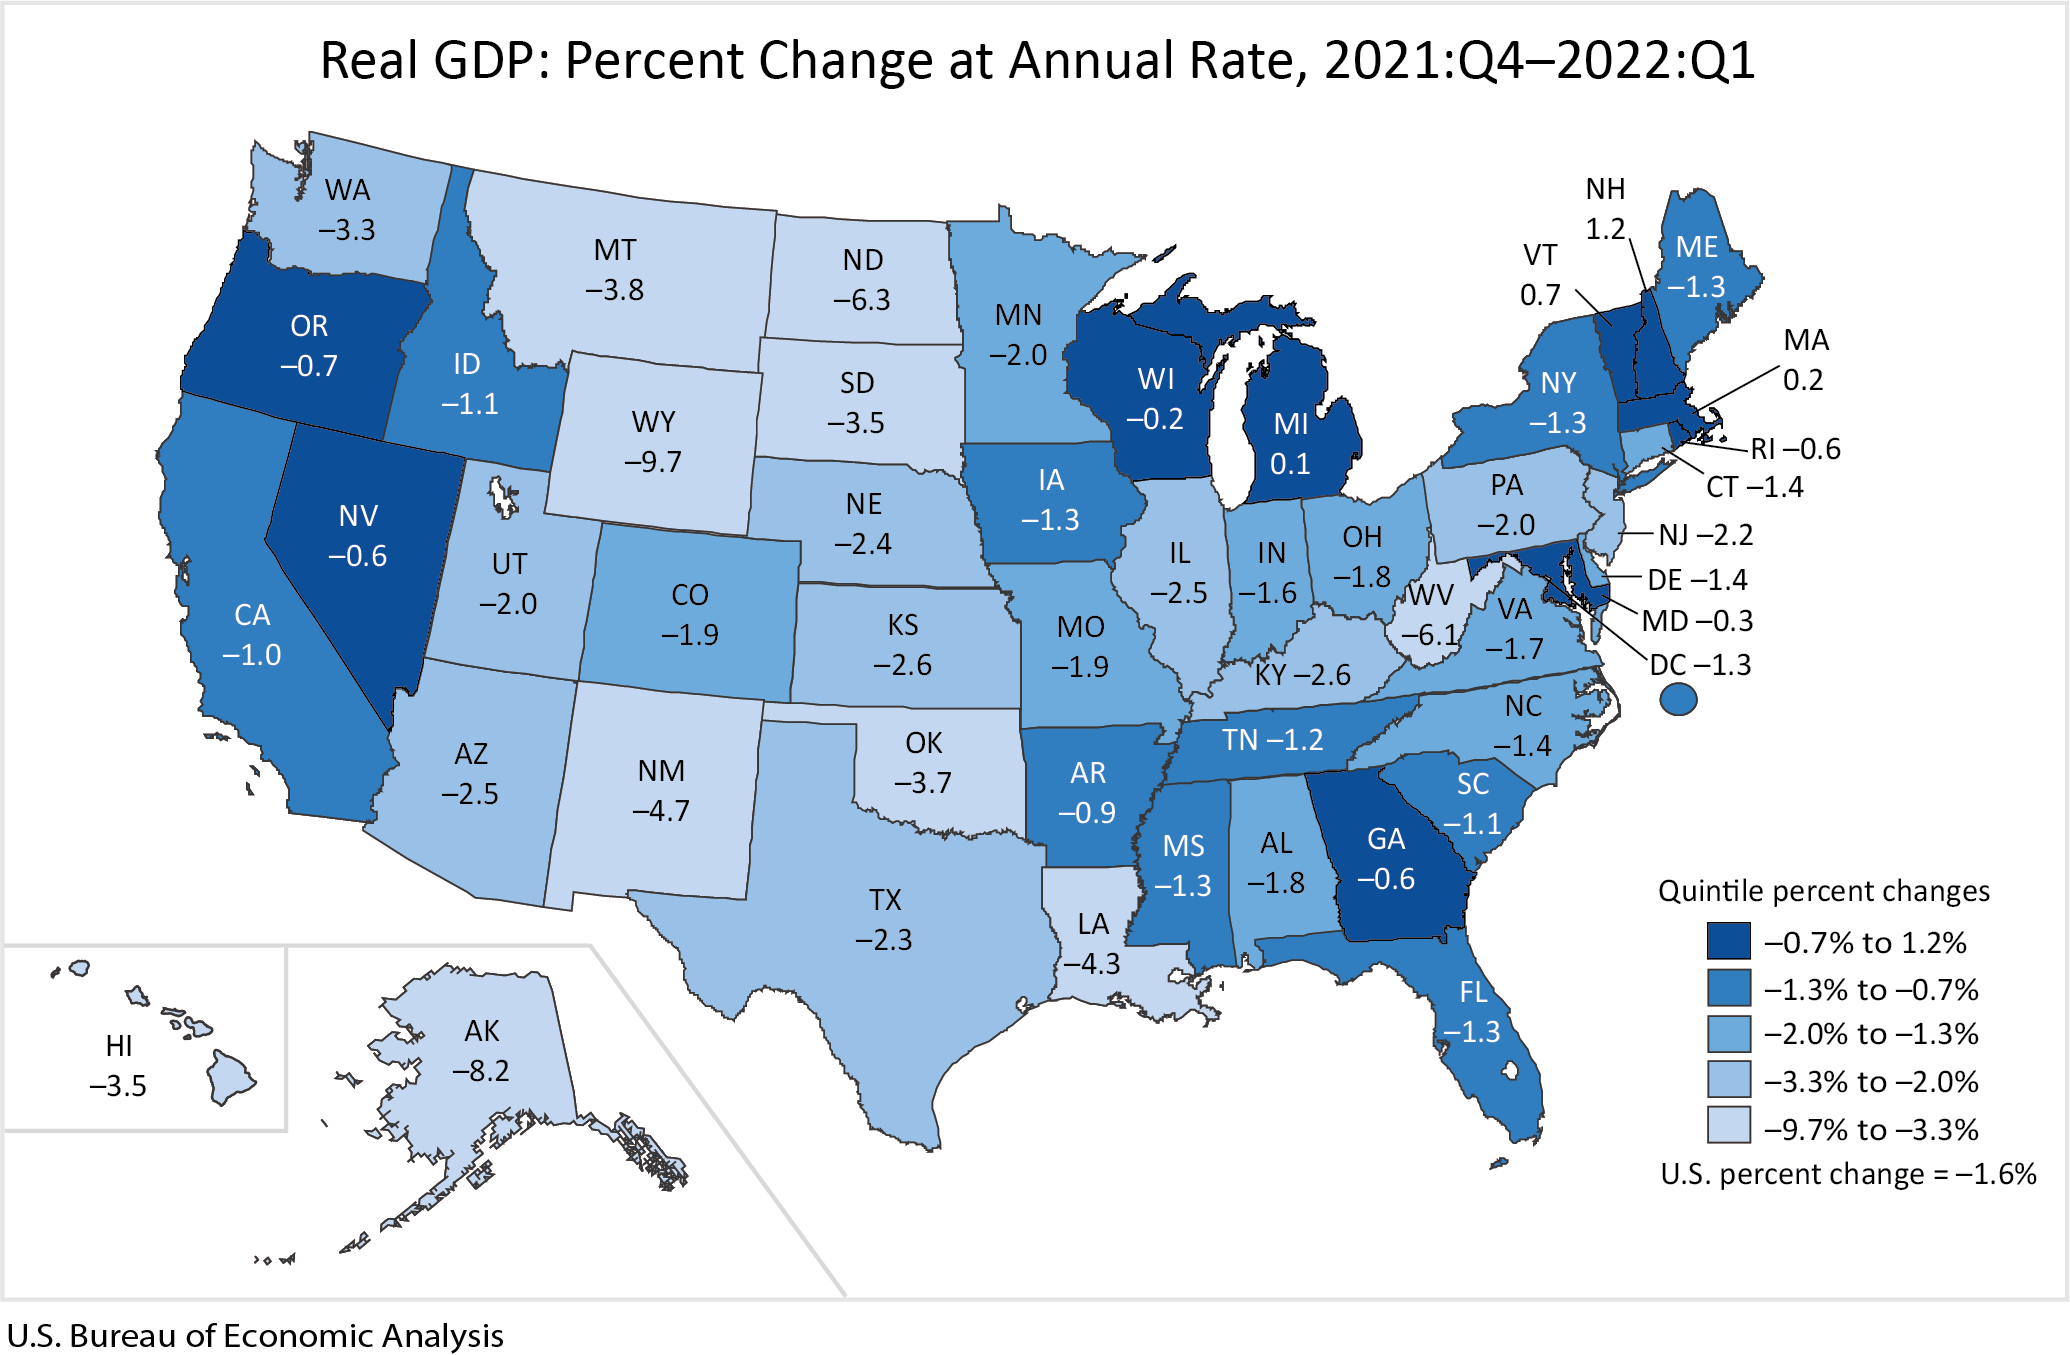
\includegraphics[width=\textwidth]{images/qgdpstate0622.png}
\end{center}

\end{frame}

%------------------------------------------%
% Research Question
%------------------------------------------%

\begin{frame}{Research Question}

\begin{center}
\begin{minipage}{0.9\linewidth}
\begin{Block}{Hypotheses}

\vspace{0.5\baselineskip}

\begin{itemize}
\item Is there a relationship between a state permitting adult-use cannabis and its GDP?

\vspace{0.75\baselineskip}

\item If a state permits adult-use, does the number of retailers per capita affect its GDP?

\vspace{0.75\baselineskip}


\end{itemize}

\end{Block}
\end{minipage}
\end{center}

\begin{center}
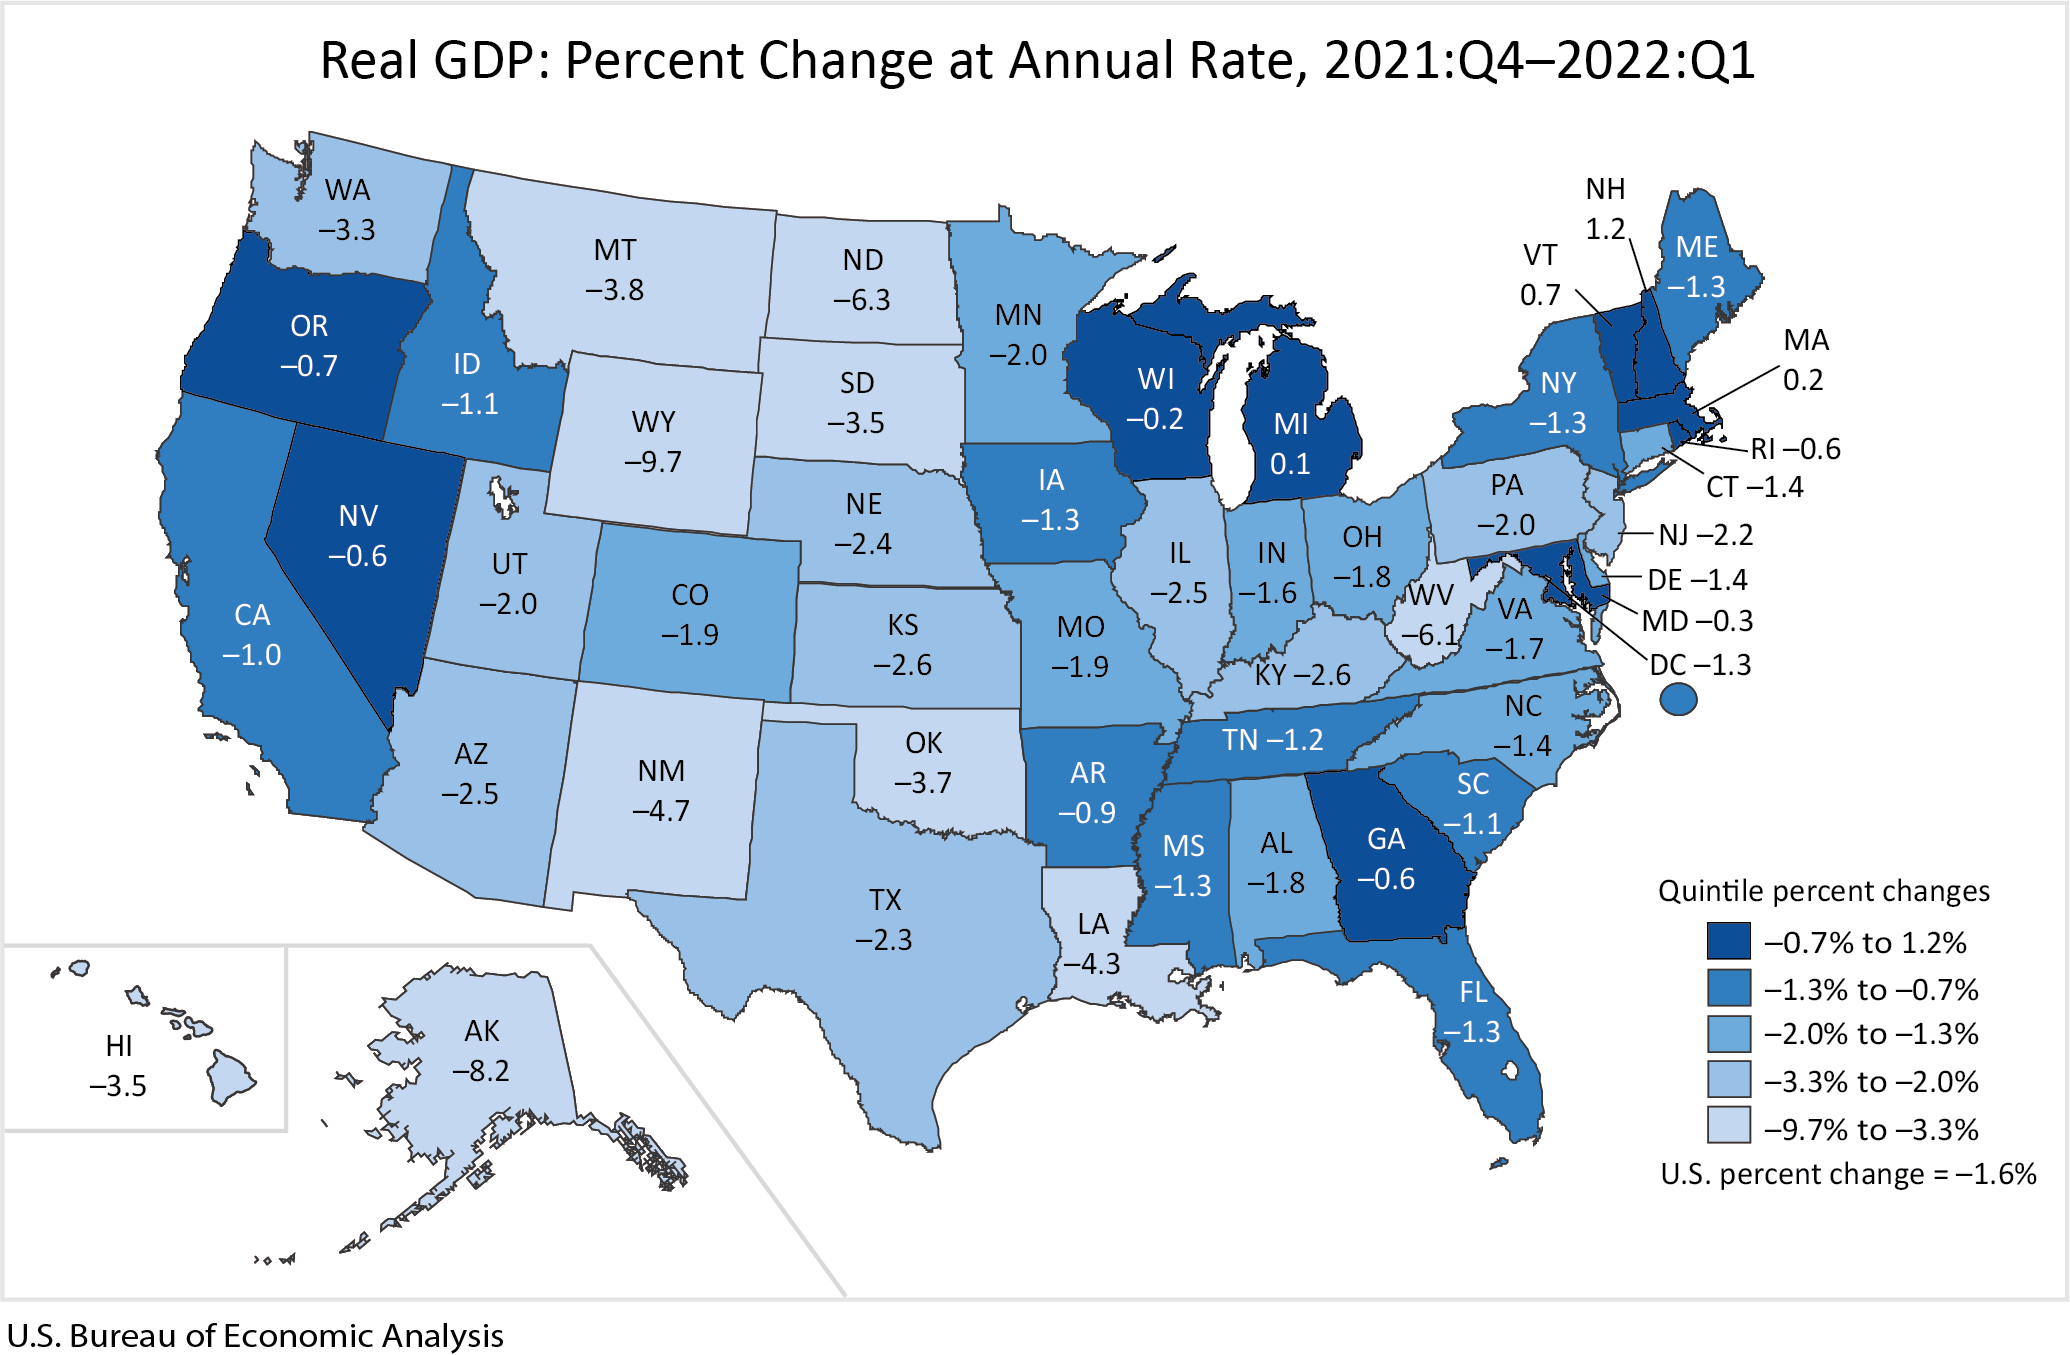
\includegraphics[width=0.5\textwidth]{images/qgdpstate0622.png}
\end{center}

\end{frame}

%------------------------------------------%
% Methodology
%------------------------------------------%

\begin{frame}{Methodology}

Assuming the following model,

\vspace{-0.25\baselineskip}
$$
\text{GDP}_s = \beta_0 + \beta_1D_s + \beta_2X_s + \mu_s,
$$

\vspace{0.25\baselineskip}
where
%\vspace{-0.25\baselineskip}
\begin{align*}
D_s &=
\begin{cases}
0 \text{ if adult-use is not permitted},\\
1 \text{ if adult-use is permitted},
\end{cases} \\
X_s & \text{ is number of retailers per capita in state } s,
\end{align*}

we can interpret:

\vspace{0.5\baselineskip}
\begin{itemize}

\item $\beta_1$ as the expected change in GDP from a state permitting adult-use cannabis,

\vspace{0.75\baselineskip}

\item $\beta_2$ as the expected change in GDP from an increase in 1 retailer per capita (100,000 people).

\end{itemize}

\end{frame}

%------------------------------------------%
% Data
%------------------------------------------%

\begin{frame}{Data}

States where adult-use is permitted:
\vspace{0.75\baselineskip}
\begin{itemize}
\begin{minipage}{0.4\linewidth}
\small
    \item Alaska
    \item Arizona
    \item Colorado
    \item Connecticut
    \item Illinois
    \item Maine
    \item Massachusetts
    \item Michigan
\end{minipage}
\begin{minipage}{0.4\linewidth}
\small
    \item Montana
    \item New Mexico
    \item Nevada
    \item New Jersey
    \item Oregon
    \item Rhode Island
    \item Vermont
    \item Washington
\end{minipage}
\end{itemize}

\vspace{0.75\baselineskip}
States where adult-use will soon be permitted:
\vspace{0.25\baselineskip}
\begin{itemize}
\small
\item New York
\item Virginia
\item D.C.?
\end{itemize}

\end{frame}

%------------------------------------------%
% Takeaway
%------------------------------------------%
\section{Takeaway}

\begin{frame}{}

\vspace{0.5\baselineskip}

\begin{center}
\begin{minipage}{3.85in}

% Thank you.

\includegraphics[width=.25in]{images/prayer.png} {\Large \textbf{Thank you for coming.}}\\[-0.75\baselineskip]

\begin{center}
\begin{minipage}{0.75\linewidth}
\begin{Block}{Insight of the Day}

\vspace{0.5\baselineskip}

\begin{itemize}
\item The squeaky wheel gets the oil!
\vspace{0.75\baselineskip}

\end{itemize}

\end{Block}
\end{minipage}
\end{center}

\vfill

\end{minipage}
\end{center}

\vspace{0.5\baselineskip}

{\large What is on your mind for next week?}\\

\end{frame}


%------------------------------------------%
% Fin.
%------------------------------------------%
\end{document}
